\section{Frequency analysis}
\label{sec:analysis}

In this following section an analysis will be made of the sound made by a car motor, windmill, EKG, breaking wine glass and four different genres of music. 
The approach of this analysis will be to plot the signal in the time domain, the fourier transformed signal and then som applied functions described in section \ref{sec:theory}.


\subsection{Car engine}

In figure \ref{fig:Car_time} a plot of the original signal is seen. This has been made using the audioread, length and plot functions described in section \ref{sec:functions}. 

\begin{figure}
	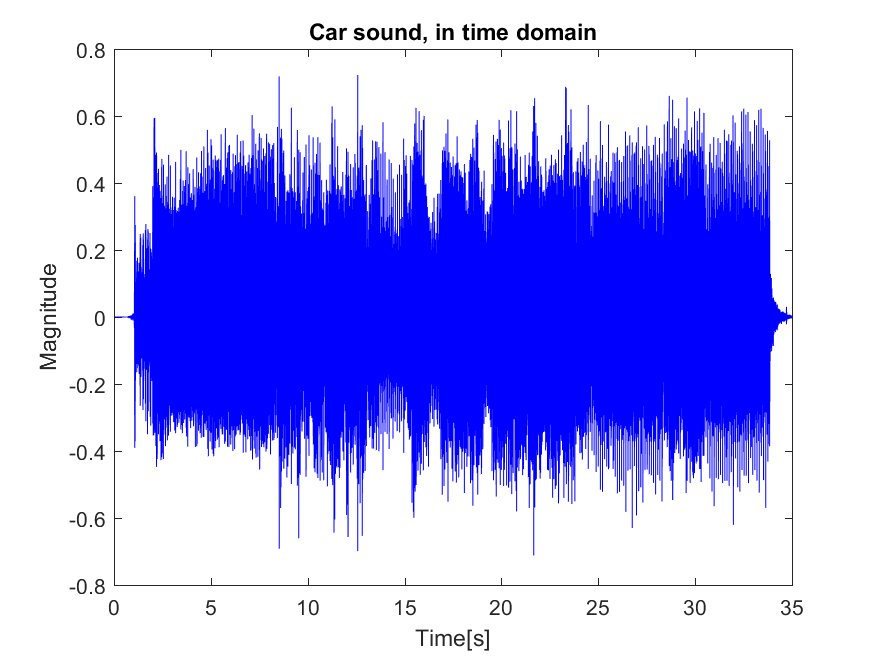
\includegraphics[width=\textwidth]{code/Car_figure1.png}
	\caption{Car signal in time domain}
	\label{fig:Car_time}
\end{figure}

\subsubsection{DFT}
The DFT of the car signal 

\begin{figure}
	\centering
	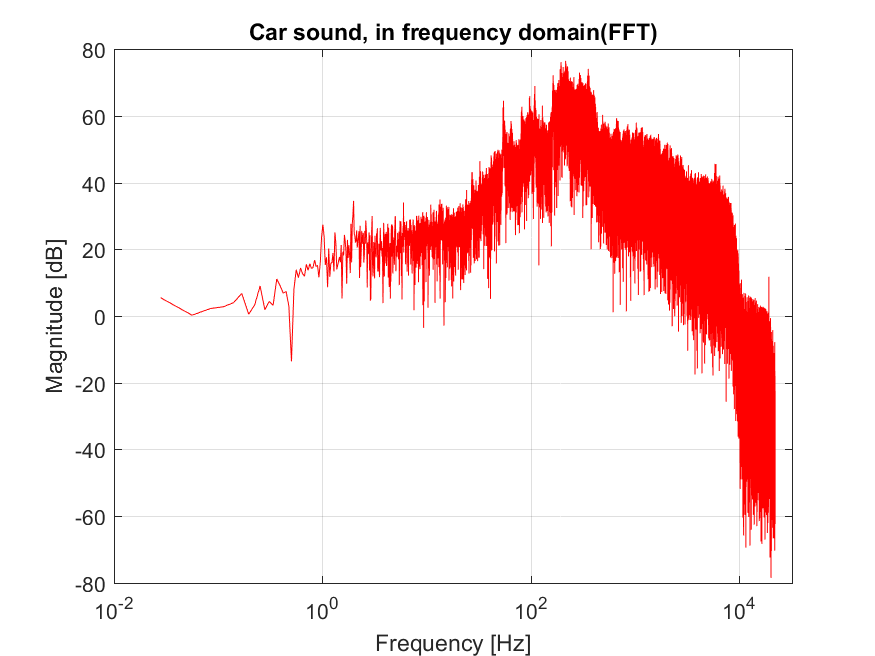
\includegraphics[width=\textwidth]{code/Car_figure2.png}
	\caption{}
	\label{fig:Car_DFT}
\end{figure}




\subsubsection{Analysis}




\subsubsection{Conclusion}

\subsection{Noise from a windmill}
\subsubsection{DFT}

\subsubsection{Analysis}

\subsubsection{Conclusion}

\subsection{EKG}
\subsubsection{DFT}

\subsubsection{Analysis}

\subsubsection{Conclusion}

\subsection{Breaking wine glass}
\subsubsection{DFT}

\subsubsection{Analysis}

\subsubsection{Conclusion}

\subsection{Music}
\subsubsection{DFT}

\subsubsection{Analysis}

\paragraph{Genre 1}

\paragraph{Genre 2}

\paragraph{Genre 3}

\paragraph{Genre 4}

\subsubsection{Conclusion}

\section{Further analysis of signals}
\label{sec:analysisOfSignals}
Eksperimenter med udglatning, zero-padding og windowing 